% THIS IS AN EXAMPLE DOCUMENT FOR VLDB 2012
% based on ACM SIGPROC-SP.TEX VERFION 2.7
% Modified by  Gerald Weber <gerald@cs.auckland.ac.nz>
% Removed the requirement to include *bbl file in here. (AhmetSacan, Sep2012)
% Fixed the equation on page 3 to prevent line overflow. (AhmetSacan, Sep2012)

\documentclass{vldb}
\usepackage{geometry}
\usepackage{balance}  % for  \balance command ON LAST PAGE  (only there!)

\usepackage{soul}
\usepackage{pdfpages}
\usepackage{booktabs} % For formal tables
\usepackage{tablefootnote}
\usepackage[hidelinks]{hyperref}
\usepackage{algorithm}
\usepackage{algpseudocode}
\usepackage{csquotes}
\usepackage{tabularx}
\usepackage{graphicx}
\usepackage{caption}
\usepackage{subcaption}
\usepackage{array}
\newcolumntype{H}{>{\setbox0=\hbox\bgroup}c<{\egroup}@{}}
\usepackage{lipsum}
%\usepackage{balance} % \usepackage{balance} in the beginning of the latex document, and then add \balance somewhere in the left column text of the last page.
%\usepackage{flushend} % this gives bibliography wrong orders
\usepackage{arydshln}
\usepackage{xcolor}
\usepackage{url}

\usepackage{multicol}

\usepackage{tikz}
\usetikzlibrary{shapes.geometric,calc}

\newcommand\score[2]{
	\pgfmathsetmacro\pgfxa{#1+1}
	\tikzstyle{scorestars}=[star, star points=5, star point ratio=2.25, draw,inner sep=0.15em,anchor=outer point 3]
	\begin{tikzpicture}[baseline]
	\foreach \i in {1,...,#2} {
		\pgfmathparse{(\i<=#1?"gray":"white")}
		\edef\starcolor{\pgfmathresult}
		\draw (\i*1em,0) node[name=star\i,scorestars,fill=\starcolor]  {};
	}
	\pgfmathparse{(#1>int(#1)?int(#1+1):0}
	\let\partstar=\pgfmathresult
	\ifnum\partstar>0
	\pgfmathsetmacro\starpart{#1-(int(#1))}
	\path [clip] ($(star\partstar.outer point 3)!(star\partstar.outer point 2)!(star\partstar.outer point 4)$) rectangle 
	($(star\partstar.outer point 2 |- star\partstar.outer point 1)!\starpart!(star\partstar.outer point 1 -| star\partstar.outer point 5)$);
	\fill (\partstar*1em,0) node[scorestars,fill=gray]  {};
	\fi
	
	,\end{tikzpicture}
}



\newtheorem{problem}{Problem}
\newtheorem{theorem}{Theorem}
\newtheorem{definition}{Definition}
\newtheorem{corollary}{Corollary}
\newtheorem{lemma}{Lemma}
\newtheorem{reduction}{Reduction}









% Include information below and uncomment for camera ready
\vldbTitle{Finding group Steiner trees in vertex-weighted graphs: approximations and applications}
\vldbAuthors{whoever, whoever, whoever, whoever, whoever, and whoever, whoever, whoever, whoever, whoever}
\vldbDOI{https://doi.org/10.14778/xxxxxxx.xxxxxxx}
\vldbVolume{xx}
\vldbNumber{xxx}
\vldbYear{2020}

\begin{document}
	
	%\settopmatter{printacmref=false}
	
	\sloppy

	
	\newpage
	\pagenumbering{arabic}
	\setcounter{page}{1}
	% ****************** TITLE ****************************************

	% possible, but not really needed or used for PVLDB:
	%\subtitle{[Extended Abstract]
	%\titlenote{A full version of this paper is available as\textit{Author's Guide to Preparing ACM SIG Proceedings Using \LaTeX$2_\epsilon$\ and BibTeX} at \texttt{www.acm.org/eaddress.htm}}}
	
	% ****************** AUTHORF **************************************
	
	% You need the command \numberofauthors to handle the 'placement
	% and alignment' of the authors beneath the title.
	%
	% For aesthetic reasons, we recommend 'three authors at a time'
	% i.e. three 'name/affiliation blocks' be placed beneath the title.
	%
	% NOTE: You are NOT restricted in how many 'rows' of
	% "name/affiliations" may appear. We just ask that you restrict
	% the number of 'columns' to three.
	%
	% Because of the available 'opening page real-estate'
	% we ask you to refrain from putting more than six authors
	% (two rows with three columns) beneath the article title.
	% More than six makes the first-page appear very cluttered indeed.
	%
	% Use the \alignauthor commands to handle the names
	% and affiliations for an 'aesthetic maximum' of six authors.
	% Add names, affiliations, addresses for
	% the seventh etc. author(s) as the argument for the
	% \additionalauthors command.
	% These 'additional authors' will be output/set for you
	% without further effort on your part as the last section in
	% the body of your article BEFORE References or any Appendices.
	

	
	%\balance
	

	
	\section*{graph\_hash\_of\_mixed\_weighted} 
	


\begin{figure} [!t]
	\vspace{0.1cm}
	\centering
	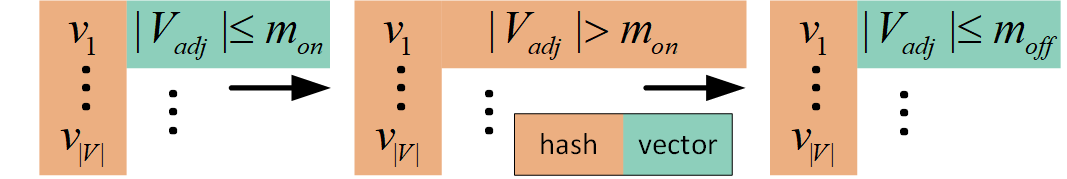
\includegraphics[width=0.46\textwidth]{adj_list}
	%\setlength{\belowcaptionskip}{-3pt}
	\caption{A non-conventional adjacency list. We store vertices $v_1, \cdots, v_{|V|}$ in a hash. Let $V_{adj}$ be the set of adjacent vertices of $v_1$. $m_{on},m_{off}$ are two values, and $m_{on} \geq m_{off}$. Initially, if $|V_{adj}| \leq m_{on}$, we store $V_{adj}$ in a vector. After adding edges, if $|V_{adj}| > m_{on}$, we store $V_{adj}$ in a hash. After removing edges, if $|V_{adj}| \leq m_{off}$, we store $V_{adj}$ in a vector.}
	\label{Figure: adj_list}
\end{figure}

\enquote{graph\_hash\_of\_mixed\_weighted} is a non-conventional adjacency list of mixed hashes and vectors to store an undirected and weighted graph $G$ (see Figure \ref{Figure: adj_list}). %We provide the C++ header files of this adjacency list at *. 
In this adjacency list, we use a hash to store all vertices. By doing this, we can access every vertex within $O(1)$ time. We set two constant values $m_{on},m_{off}$ such that $m_{on} \geq m_{off}$.  Let $V_{adj}$ be the set of adjacent vertices of vertex $v_1$. Initially, if $|V_{adj}| \leq m_{on}$, we store $V_{adj}$ in a vector. After adding edges, if $|V_{adj}| > m_{on}$, we store $V_{adj}$ in a hash. After removing edges, if $|V_{adj}| \leq m_{off}$, we store $V_{adj}$ in a vector again. The purpose of using vectors and hashes to store small and large sets of adjacent vertices respectively is to employ both the small memory consumption of vectors and the small time complexities of hashes. The space time complexity of this adjacency list is $O(|V|+|E|)$.  
Since the size of a vector in this adjacency list is constrained by $m_{on}$, the time complexity of adding or removing an edge is $O(1)$. 












%	\bibliographystyle{abbrv}
%	{\small
%		\bibliography{YahuiBibIEEE}}
	

\end{document}
